%!TEX root =  secondDraft.tex

\chapter[Background]{Background}

We want to create grounded Bayesian Networks for reasoning with evidence. This can be done by creating multi-agent simulations, and building Bayesian Networks based on the events in these simulations. In this section, the relevant background is laid out on reasoning with evidence, Bayesian Networks, and multi-agent simulations.

\section{Reasoning with evidence}
We consider three main directions in the field of reasoning with evidence within law \citep{Verheij2015}. The first direction is via argumentation approaches, where hypotheses and evidence are represented as propositions that attack or support each other. The second direction is via scenario approaches, where more-or-less coherent hypotheses are combined into stories \citep{Pennington1993}, \citep{wagenaar1993}, which are supported with evidence. The third direction is via probabilistic approaches, where hypotheses and evidence are assigned probabilities, and the relation between hypothesis and evidence is represented with conditional probability. There are also be hybrids that combine or synthesise aspects of each approach, see, for example: \citep{Bex2010} and \citep{Timmer2016}. This project does not consider the argumentative approach, and is mainly based on the work of Vlek \citep{Vlek2015}, \citep{Vlek2016} and Fenton \citep{Fenton2012}, \citep{Fenton2019}. The networks in these papers describe whole criminal situations (scenarios), but use Bayesian Networks and hence have a probabilistic component.


\section{Bayes and Bayesian Networks}

We have already seen the power of Bayes's law in the introduction. It tells us how much we have to change our belief in a hypothesis once we find a piece of evidence. To do this, we need to have probabilistic or frequentist information about the likelihood ratio and the prior. 

Bayesian reasoning, without Bayesian Networks, have been used by Dahlman in `event trees', specifying different branches of combinations and their probabilities \citep{dahlman2020}.

However, just using Bayes law is very difficult, because sometimes we want to condition on multiple pieces of evidence. Doing all the calculations is tedious, hence we use the computational tools called Bayesian Networks. 

Bayesian Networks can represent aspects of a criminal case or can attempt a scenario-like hybrid and represent the entire case - modelling actual crime cases \citep{Kadane1996}, \citep{Fenton2019},  cases from fiction \citep{Fenton2012} or fictionalized crime cases \citep{vanLeeuwen2019}. In situations where the network represents aspects, the nets model DNA or blood-spatter evidence, for methods see \citep{Meester2021}. 

Bayesian Networks can be built by hand, by experts or academics, in (proprietary) software like AgenaRisk or Hugin. They can also be built by hand in PyAgrum \citep{pyagrum2020}, a free Python software package, which does not have a GUI but has everything else. In this project, PyAgrum was used. Alternatively, Bayesian Networks can be automatically constructed from large datasets - PyAgrum also offers the opportunity for that. %Automated Bayesian Network building is not plausible in the legal-evidence domain, because the data that we need is notoriously sparse.
%However, since we're using simulations to investigate the Bayesian Approach, we can generate a near infinite amount of information, and then we use this information to build the network, such as we might use data on health markers to predict kidney failure (medical domain - pretty sure this is the standard example). So automated building tools come in handy. In this project I only used the K2 algorithm, because you can add temporal information to it.

Bayesian Networks are a promising tool, but there are a lot of open questions:
\begin{enumerate}
\item The use of Bayesian Networks is not straightforward, neither for the builder or for the interpreter. From \citet{deKoeijer2020}: it is complex, time-consuming, hard to explain, and, the `repeatability [...] leaves much to be desired. Node definitions and model structures are often directed by personal habits, resulting in different models for the same problem, depending on the expert'.
\item The granularity of the network - how do we know which nodes hypotheses and pieces of evidence to include? Ideally we would model as detailed as possible, but as we increase the number of nodes, we increase the complexity, which increases the probability of mistakes, and the time spend on the network.
\item The links: how do we know which events depend on each other?
\item The numbers - there's not just subjectivity in selecting the nodes, and drawing the links, but the probabilities that we have to fill in into the cpt themselves are the most obvious stumbling block. We can identify that there has to be some sort of correlation between `smoke' and `fire', but how to express this in numbers? Fenton argues that we're just making something explicit that we would otherwise have left implicit. But what are the consequences of making something explicit, but doing it wrongly? How robust is the network against imprecise or wrong frequencies? If we use frequencies (or subjective probabilities based on frequencies), how do we decide what set of events is included when we start to count (this is the problem of the reference class, see \citep{Allan2007}, \citep{colyvan2001}). Probabilities can be pure frequencies, or can be subjectively elicited from experts \citep{renooij2001}, \citep{Druzdzel2000}.
\end{enumerate}





\subsection{Evaluating Bayesian Networks}

There is a precedent for building Bayesian Networks to model reasoning with evidence in criminal cases, although these methods have not been used in court. However, even though there are methods for building these networks, it is unclear how to determine how we can validate these networks.

In more data-rich domains, where we train Bayesian Networks on large amounts of frequency data, we can estimate the accuracy of the networks by cross-validation. We construct the network based on some subset of the data and then use the rest of the data as a test, to see whether the prediction of the network is correct, given some input (a split of 80/20 for train/test is common) (good practice Chen) This approach prevents overfitting, where the network might perform well on some subset of input, but perform worse on some other, unrepresented subset.

However, this approach towards BN validity through accuracy is implausible, given the circumstances of court cases. The court cases involve one-of-a-kind events (schum, 1982), which means that it is unlikely that we can find frequency data on most of the nodes present in our Bayesian Network. This is why the probabilities in these Bayesian Networks in court cases are subjective probabilities, either elicited from experts or estimated by the modeller (sometimes based on real data).

This does not mean that there are no methods of evaluating these Bayesian Networks, however. Evaluation of the Bayesian Networks for criminal cases as found in the existing literature confine themselves to two approaches:

\begin{enumerate}

\item Sensitivity analysis

Sensitivity analysis tests the effect of small parameter changes on the outcome of the network. This is useful if the outcome of the network hinges on elicited or subjectively estimated probabilities. 

\item Cumulative evidence on one set of evidence

In this approach, the modeller selects all evidence nodes, and start to enter the evidence that was established during the trial. This results in a cumulative posterior probability on the outcome node. In this process, we can see how much each piece of evidence contributes to our overall final belief in the posterior.

\end{enumerate}

However, what we see with this cumulative evidence approach, is that we are only testing one set of evidence. Both Vlek and Fenton only test the cumulative probability of the output node by turning on the evidence nodes that the court has found. However, this is a risky move, since this might lead to overfitting the probabilities in the CPTs, so that the network seems to reflect the right `evidence strength' on the selected set of evidence, but misrepresenting other combinations of evidence. An example of this overfitting can be found in \citep{vanLeeuwen2019}, which is biased towards the scenario that the suspect is guilty. In Figure~\ref{love}, we see a situation where a certain set of evidence is entered into the network. The outcome of the network is, that the suspect is guilty. But the evidence that is entered into this network, would not rationally support this conclusion: there is no body, no signs of violence, no car with bloodstains, to evidence of existing conflict... The only evidence that the prosecution has, are some phone calls, and perhaps some testimony of the suspect that does not match medical reality. Even with this scant set of evidence, the Bayesian Network would decide to convict.

\begin{figure}[htbp]
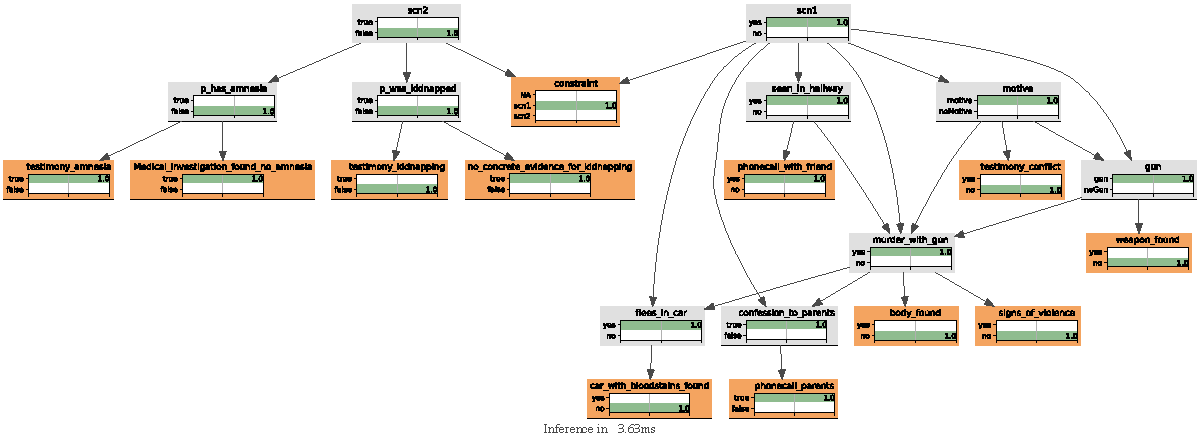
\includegraphics[width=\linewidth]{images/oldnetwork.pdf}
\caption{Example of subjective probability estimation resulting in overfitting}
\label{love}
\end{figure}%

This illustration shows that it is necessary to consider all possible combinations of evidence. If we have tunnel vision and only focus on the set of evidence that is found in court, we might create a network that overfits. If we want to take the premise behind BNs seriously, we have to create a network that gives sensible results for all possible combinations of evidence valuations - and not just the valuation of the evidence that are established in court.





\section{Agent simulations}
We can create such a data-generating environment for criminal cases by the use of multi-agent simulations. In a multi-agent simulation, agents observe and interact with their environment. The environment and the agent behaviour is fully controlled by its programming and all randomness can be accounted for. This means that we know exactly with which frequencies fully-specified events occur. Running the simulation multiple times generates a lot of data, which will serve as input to automatically build a Bayesian Network from data. This means we use a multi-agent simulations as a ground for our theory-testing. In this project, the simulations will be programmed in Python using the MESA framework  \citep{mesa2020}.


Multi-agent simulations have been used to investigate the criminal domain and to test out sociological theories. By creating spatially explicit simulations, the complex interactions of agents with their locations can be represented better than in traditional models - these agent-based models can model criminal hotspots \citep{Gerritsen2008}, theories of behaviour \citep{Gerritsen2015}, and police strategies in urban crime \citep{Zhu2021}. Weaknesses identified with multi-agent models for criminological research are insufficiently complex models, unclarity on the effect of temporal resolution, and lack of a systemic approach \citep{Zhu2021}.





 \section{Conclusion}

The two main ideas are Bayesian reasoning, specifically as implemented in Bayesian Networks, and computational simulations of agents. The simulation is supposed to be the grounding for the Bayesian Networks.

But why do we want to use Bayesian Networks in the first place? In the best possible case, a Bayesian Network would help us to make the correct reasoning steps, telling us exactly how to weigh each piece of evidence in the grand scale of the simulated crime. This is a normative approach - it's telling us how to reason, but it is not (and not meant to be) an empirical approach. Bayesian networks are not a reflection of `how people actually reason' - If you open up our minds, you won't see Bayesian Networks in there. One of the problems for normative models in decision making \citep{colyvan2013}, is that we can only test how well our normative models work, if we already know what a good outcome would be. In a sense, we're doing experimental model testing for normative Bayesian Networks in this project.


%\begin{quote}
%"Unfortunately, as we recognize, we can never ask how correct or accurate is a person's assessment of the probative weight either of an item of evidence or a collection of evidence given at 	trial. Such evidence involves unique or one-of-a-kind events, and each fact finder evaluates the evidence according to personal 	strategies based upon a unique matrix of prior experience. In short, there is no "true" or "correct" probative weight for any item 	or collection of evidence; still, even though we cannot measure the accuracy of probativity assessment, we can, under certain 	circumstances evaluate the consistency or coherence of such assessments."
%\end{quote}



% This is not necessarily a bad thing - we put our (betting) money where our mouth is and assign numerical precise probabilities to situations that we preciously only had vague intuitions for. However, this brings about the veil of objectivity. By giving a probability to your intuitions, you have made your intuitions more precise and you can now reason with them, update on evidence using Bayes Law, and everything's great. In some domains, this is obviously okay. If you want to bet cents on world events and walk that fine line between calibration and discrimination for fun and profit, that's no problem.  After all, there are incentives to abstain from the unclear, the stuff that might not have a specified answer, the vague. But when we are talking about using evidence in law, we are talking about exactly that domain - we're not making predictions about the price of oil in 6 months, or the outcome of the French election, with clear outcomes, clear procedures for measurement. Instead, we're trying to make predictions about crimes and crime scenarios, which are a lot vaguer, and strangely unobservable at times - things like motives, or behaviours that happen under specific circumstances, interlocking stuff with complex dependencies. We all have intuitions about evidence strengths in vague situations, but they are more difficult to make precise than the traditional `forecasting' events. So trying to assign probabilities without a clear method of calibration, makes that they will be imprecise.

